\documentclass[12pt, letterpaper]{article}
\usepackage{times}
\usepackage{graphicx}
\usepackage{import}
\usepackage{fancyhdr}
\usepackage{wrapfig}
\usepackage[utf8]{inputenc}
\usepackage[hidelinks]{hyperref}
\usepackage{subcaption}
\usepackage{pdfpages}
\usepackage{enumitem}
\usepackage{titling}
\pagestyle{fancyplain}% <- use fancyplain instead fancy
\fancyhf{}
\addtolength{\headheight}{15pt}
\fancyhead[L]{Cyber Security: PVI - Konstantinos Poumpouridis}% <- added
\fancyhead[R]{488394}
\fancyfoot[C]{\thepage}
%\renewcommand\headrulewidth{0pt}% default ist .4pt
\renewcommand{\plainheadrulewidth}{.4pt}% default is 0pt
\title{Personal Project: Vulnerability Investigation}
\author{Konstantinos Poumpouridis}
\date{05/04/2023}
\pagenumbering{arabic}
% set up \maketitle to accept a new item
\predate{\begin{center}\placetitlepicture\large}
\postdate{\par\end{center}}

% commands for including the picture
\newcommand{\titlepicture}[2][]{%
  \renewcommand\placetitlepicture{%
    \includegraphics[#1]{#2}\par\medskip
  }%
}
\newcommand{\placetitlepicture}{} % initialization
\begin{document}
\titlepicture[width=1.5\textwidth]{fotos/PVI/Fritzbox/Fritzfrontpage.jpeg}
\maketitle
\thispagestyle{empty}

\newpage
\section{Changelog}
    \begin{table}[htbp]
        \begin{tabular}{|l|l|l|}
            \hline
            Version & Changes         & Date   \tabularnewline \hline
            0.1     & Initial version & 05/04/23 \tabularnewline \hline
            0.2     &  First draft & 20/04/23 \tabularnewline \hline
            0.3     &  Added more backstory and conclusion & 25/04/23 \tabularnewline \hline
            0.4     &  Added legality, the testing and restructured my headers & 27/04/23 \tabularnewline \hline
        \end{tabular}
    \end{table}
\newpage
\tableofcontents
\newpage

\section{Introduction}
This investigation provides an overview of the vulnerability investigation conducted on the SMBv1 protocol used by the Windows operating system. SMBv1 has been known to have several vulnerabilities that can be exploited by attackers to gain unauthorized access to systems and data. In total, there are 36 CVE's related to SMBv1 that can be used to compromise Windows systems.

\section{Background}
Since that, I've had a lot of Fritz products and a spare FRITZ!Box to try on and in the specification they offer FRITZ!NAS in their os but one issue is that it only supports SAMBA Version 1 which is considered not safe anymore by today's standard.

\subsection{History of SMB}
The Server Message Block (SMB) protocol was created in 1983 by Barry A. Feigenbaum at IBM. It was originally made to enable file and printer sharing among devices on a network of systems running IBM's OS/2, SMB also provided an authentication. Microsoft and 3Com later implemented SMB in LAN Manager for OS/2 in 1987, using the NetBIOS. SMB was later implemented in Windows NT 3.1 by Microsoft and has been continually updated to work with newer features, like TCP/IP and NetBT. 

\subsubsection{SMB 1}
As mentioned SMB 1 was created in 1983 by Barry A. Feigenbaum. It was officially supported by Microsoft until June 2013.
\subsubsection{CIFS}
This was created in 1996 when Sun Microsystem announced WebNFS. Microsoft changed SMB to Common Internet File System or CIFS. This brought lot of features like including symbolic links, hard links, larger file sizes and support connections over TCP (port 445).

\subsubsection{SMB 2.0}
SMB 2.0 or SMB2, Microsoft introduced a new version of the protocol in 2006 on Windows Vista and Windows Server 2008

\subsubsection{SMB 2.1}
Adds more features and performance optimization. It got deployed alongside Windows 7 and Windows Server 2008 R2.

\subsubsection{SMB 3.0}
SMB 3.0 (previously named SMB 2.2) was introduced with Windows 8 and Windows Server 2012. It brought several significant changes that are intended to add functionality and improve SMB2 performance. It adds extra features.

\hfill\break
the SMB Direct Protocol 
SMB Multichannel (multiple connections per SMB session) and
SMB Transparent Failover
It also introduces several security enhancements, such as end-to-end encryption and a new AES based signing algorithm.[

\subsubsection{SMB 3.0.2}
SMB 3.0.2 (known as 3.02 at the time) was introduced with Windows 8.1 and Windows Server 2012 R2 in those and later releases, the earlier SMB version 1 can be optionally disabled to increase security
\subsubsection{SMB 3.1.1}
It comes to Windows 10 and Windows Server 2016.It supports AES-128 and SHA-512. And security is mandatory right now.

\subsubsection{Samba}
Which is an open source version of SMB which GNU/linux uses.

\subsubsection{Netsmb}
NSMB (Netsmb and SMBFS) is a family of in-kernel SMB client implementations in BSD operating systems. It was first contributed to FreeBSD 4.4 by Boris Popov, and is now found in a wide range of other BSD systems including NetBSD and macOS. The implementations have diverged significantly ever since.
\hfill\break
\hfill\break

This information was cited in Wikipedia - Server Message Block: \url{https://en.wikipedia.org/wiki/Server_Message_Block}

\newpage

\section{Research Questions}
List your main research questions and any sub-questions that will help you to answer them. Be specific and ensure that your questions are answerable.

\subsection{Main Research question}
\begin{enumerate}
    \item What is the impact of these vulnerabilities on the security of FRITZ!Box and its users?
\end{enumerate}

\subsection{Sub Research questions}
\begin{enumerate}
    \item How do the vulnerabilities affect the confidentiality, integrity, and availability of FRITZ!Box and FRITZ!Box NAS?
    \item What are the most common types of exploits for SMB V1 
    \item Can vulnerability cause more damage to the rest of FRITZ!Box?
    \item What other devices can be affected?
    \item What can AVM (The factory) do to mitigate or prevent this?
\end{enumerate}

\newpage

\subsubsection{How do the vulnerabilities affect the confidentiality, integrity, and availability of FRITZ!Box and FRITZ!NAS?}
\hfill\break
Since SMB 1 is old and has probably been dissected by every security group it was only time that they would discontinue it. Back then security wasn't that big and or a major priority. We live now in a cyber world where people share a lot of data through the internet and into their local database/NAS.
\hfill\break
\hfill\break
The vulnerabilities of SMB 1 have existed far too long. Microsoft has vulnerabilities over 30 known 30 CVEs which tells you how unsafe it is nowadays.

\hfill\break
This vulnerability can impact the confidentiality, integrity, and availability of systems that use SMBv1, including FRITZ!NAS. An attacker who is able to exploit one of these vulnerabilities can gain unauthorized access to sensitive data and destroy it or cause the system to become unstable.
\hfill\break
\hfill\break
Sources
\begin{enumerate}
\item Microsoft. (2017). \textit{Disabling SMBv1 through Group Policy}. Retrieved from \url{https://docs.microsoft.com/en-us/security-updates/SecurityAdvisories/2017/4033453}

\item US-CERT. (2017). \textit{Alert (TA17-132A) Indicators Associated With WannaCry Ransomware}. Retrieved from \url{https://us-cert.cisa.gov/ncas/alerts/TA17-132A}
\end{enumerate}

\newpage
\subsubsection{What are the most common types of exploits for SMB V1?}

These exploits can have a significant impact on the confidentiality, integrity, and availability of systems that use SMBv1. It is recommended to disable SMBv1 and use more secure versions of the protocol to reduce the risk of exploitation.
\hfill\break
If we take the exploits from the other header and dissect them. we can see the popular methods are sending payloads or sending a malicious executable file to the target. The user cannot prevent this because there is no security in this protocol.
\break
Some of the most common types of exploits for SMBv1 include: 
\begin{itemize}
\item EternalBlue (CVE-2017-0144) - This is a vulnerability that was used in the WannaCry ransomware attack in 2017. It allows an attacker to execute arbitrary code on a remote system without authentication.
\item SambaCry (CVE-2017-7494) - This is a vulnerability that affects the Samba software, which is an open-source implementation of the SMB protocol. It allows an attacker to execute arbitrary code on a remote system.
\item {Badlock (CVE-2016-2118)} - This vulnerability affects the SMB protocol and can allow an attacker to perform man-in-the-middle attacks, steal data, or execute code on a remote system
\end{itemize}

Sources
\begin{itemize}
\item US-CERT. (2018). SMB Security Best Practices. \url{https://www.us-cert.gov/ncas/current-activity/2018/04/19/SMB-Security-Best-Practices}
\item Microsoft. (2017). Disabling SMBv1 through Group Policy. \url{https://docs.microsoft.com/en-us/security-updates/SecurityAdvisories/2017/4033453}
\item Trend Micro. (2017). Ransomware WannaCry Attacks Using NSA Exploit Leaked by Shadow Brokers. \url{https://www.trendmicro.com/en_us/research/17/h/wannacry-ransomware-used-in-global-attacks-what-we-know.html}
\item Cisco Talos. (2019). Emotet Malware. \url{https://blog.talosintelligence.com/2019/08/emotet-malware.html}
\item SANS Institute. (2016). \textit{Badlock Vulnerability}. Retrieved from \url{https://www.sans.org/security-awareness-training/blog/badlock-vulnerability}
\end{itemize}
\newpage

\subsubsection{What other devices can be affected?}
Devices that use SMBv1 are open to be exploited, including Windows machines running outdated versions of the operating system, network-attached storage (NAS) devices, and Internet of Things (IoT) devices even though it is rare since IOT is quite new which it would not make sense. Some specific examples of devices that may be affected include:

\begin{itemize}
\item FRITZ!Box NAS feature (SMBv3 is available above FRITZ!OS 6.20 but still supports SMBv1)
\item Synology NAS devices (When you use the old firmware)
\item QNAP NAS devices (Need to update to QTS 5 to be safe)
\item Western Digital My Cloud NAS devices (Older devices use SMBv1 most are in SMBv2 or higher)
\end{itemize}
\hfill\break
Sources:
\hfill\break
Info about Western Digital from: \url{https://support-en.wd.com/app/answers/detailweb/a_id/25436} and \url{https://community.wd.com/t/smbv1-and-mycloud-home/237082}
\hfill\break
Info about FRITZ!Box from: \url{https://nl.avm.de/service/knowledge-base/dok/FRITZ-Box-5490/1364_Toegang-tot-opslag-NAS-geconfigureerd-als-netwerkstation-niet-mogelijk/}
\hfill\break
Info about FRITZ!Box from: \url{https://kb.synology.com/en-global/DSM/help/DSM/AdminCenter/file_winmacnfs_win?version=7}

\newpage
\subsubsection{What can AVM (The factory) do to mitigate or prevent this?}
Since SMBv1 is very old it is recommended to be shut down so that you reduce significant security risks. SMBv2 and SMBv3 are fine it is even better if you only need SMBv3 since it came out in 2012.
\hfill\break
\hfill\break
As user:
\begin{itemize}
    \item Use the latest version of an Operating System
    \item Stay away from SMB versions 1 and 2
    \item Preferable use USB external storage's to prevent this
    \item More expensive option is to use Cloud services since they keep their protocol up to date but use a reputable cloud provider.
\end{itemize}

\section{Objectives}
The main objectives of this investigation are:
\begin{itemize}
    \item To identify vulnerabilities.
    \item To determine how much damage it can cause.
    \item To recommend preventing this vulnerability 
\end{itemize}

\newpage
\section{Methodology}
The investigation was conducted using a combination of manual and automated techniques. The following steps were taken:

\begin{itemize}
\item Conducted a literature review to understand the historical context of SMBv1 vulnerabilities.
\item Analyzed the Windows operating system to identify potential vulnerabilities related to SMBv1.
\item Used vulnerability scanning tools to identify and assess the severity of any vulnerabilities discovered.
\item Conducted penetration testing to simulate a real-world attack on the SMBv1 protocol.
\item Analyzed the results of the vulnerability testing to identify the most critical vulnerabilities that must be addressed.
\end{itemize}
\newpage
\section{Legality}
According to Rijks Overheid and Police, Any attack based on cyber is punishable on top of it is generally not allowed do General Data Protection Regulation (GDPR) or AVG Algemene Verordening Gegevensbescherming. The article is in sources but what they say is if the hacker has your data without your authorization or permission then it is called theft or cyber theft. There is a site that I've searched where they show all the punishment you can receive. I've chosen company as an example of what a hacker can receive alongside a fine.
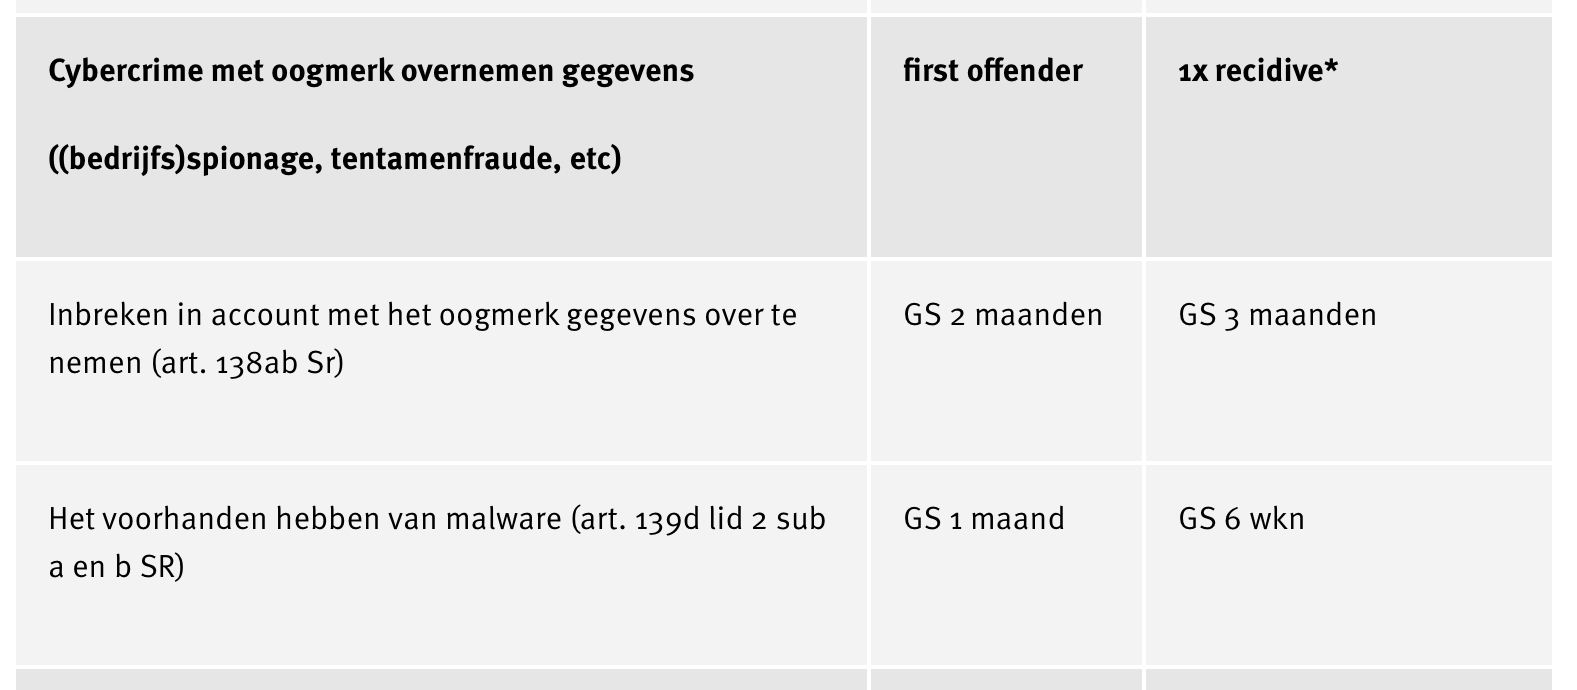
\includegraphics[width=1\textwidth]{fotos/PVI/Boete.jpeg}
\break
\emph{Dutch punishment, TS = taakstraf, GS = Gevangenis straf, \url{https://www.om.nl/onderwerpen/beleidsregels/richtlijnen-voor-strafvordering-resultaten/richtlijn-voor-strafvordering-cybercrime-2018r001}}
\hfill\break
\hfill\break
So in short yes it is illegal (duh) since it breaks multiple privacy laws and this does count as theft which is also a big no-no. Since it is a personal environment the punishments may be lower due to the total damage that you can cause being less than in a company. But still, you can get jail time for it alongside a fine depending on how much data is stolen/damaged. 
\hfill\break
\hfill\break
Sources:
\hfill\break
Info about data theft from: \url{https://www.vraaghetdepolitie.nl/politiewerk-en-boetes/boetes-en-straffen/wat-is-er-allemaal-strafbaar-online.html} 
Info about punishes for cyber attacks from: \url{https://www.rijksoverheid.nl/onderwerpen/cybercrime-en-cybersecurity/cybercriminaliteit-bestrijden}
Info about AVG theft from: \url{https://autoriteitpersoonsgegevens.nl/nl/onderwerpen/politie-en-justitie/bestrijding-van-ondermijnende-criminaliteit}
Info about punishment \url{https://www.om.nl/onderwerpen/beleidsregels/richtlijnen-voor-strafvordering-resultaten/richtlijn-voor-strafvordering-cybercrime-2018r001}

\section{Materials}
To create a test environment, I need to have the materials to run this test if it is true.
\begin{enumerate}[label=(\roman*)]
    \item FRITZ!Box 5490
    \item MSI GF63 8rc
    \item iPad Pro M1
    \item Lan cable
\end{enumerate}
\subsection{Tools}
\begin{enumerate}
    \item smbmap
    \item nmap
    \item d4t4s3c/SMBploit
    \item Fritzbox diagnostic
    \item Virtualbox/NAT
\end{enumerate}
\section{Results}

The investigation revealed several critical vulnerabilities related to SMBv1 that must be addressed immediately. The following are the most significant findings:

\begin{itemize}
\item SMBv1 does not require authentication by default, which can allow attackers to gain unauthorized access to systems.
\item SMBv1 is vulnerable to man-in-the-middle attacks, which can allow attackers to intercept and manipulate data transmitted over the protocol.
\item SMBv1 is susceptible to buffer overflow attacks, allowing attackers to execute malicious code on the targeted system.
\item SMBv1 is susceptible to denial-of-service attacks, which can cause systems to crash or become unresponsive.
\end{itemize}

\subsection{CVE's}
\includegraphics[width=1.2\textwidth]{fotos/PVI/IMG_0516.jpeg}
\break
\emph{This is the CVE list that shows SMBV1 leaks (source: https://cve.mitre.org while searching "SMBv1")}
\hfill\break
\hfill\break
After researching I've discovered that Windows still supports SMB v1 in Windows 10 but it is disabled by default. We are in SMBv3 right now with more security protocols.

\subsection{The testing}
I started to use my laptop and try to my FRITZ!Box without access to the internet but my Kali refused to connect to my FRITZ!Box router is not even on the login screen of the device.
\newpage
\textbf{This was my setup for my testing}
\hfill\break
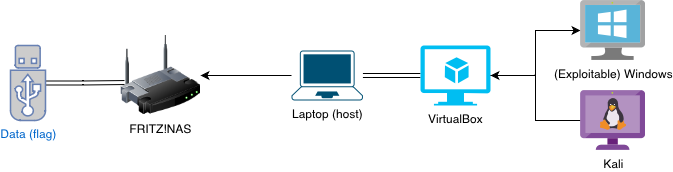
\includegraphics[width=1\textwidth]{fotos/PVI/PVI drawing.drawio.png}
\break
\emph{My drawing how I'm going to test my PVI}
\hfill\break
\hfill\break
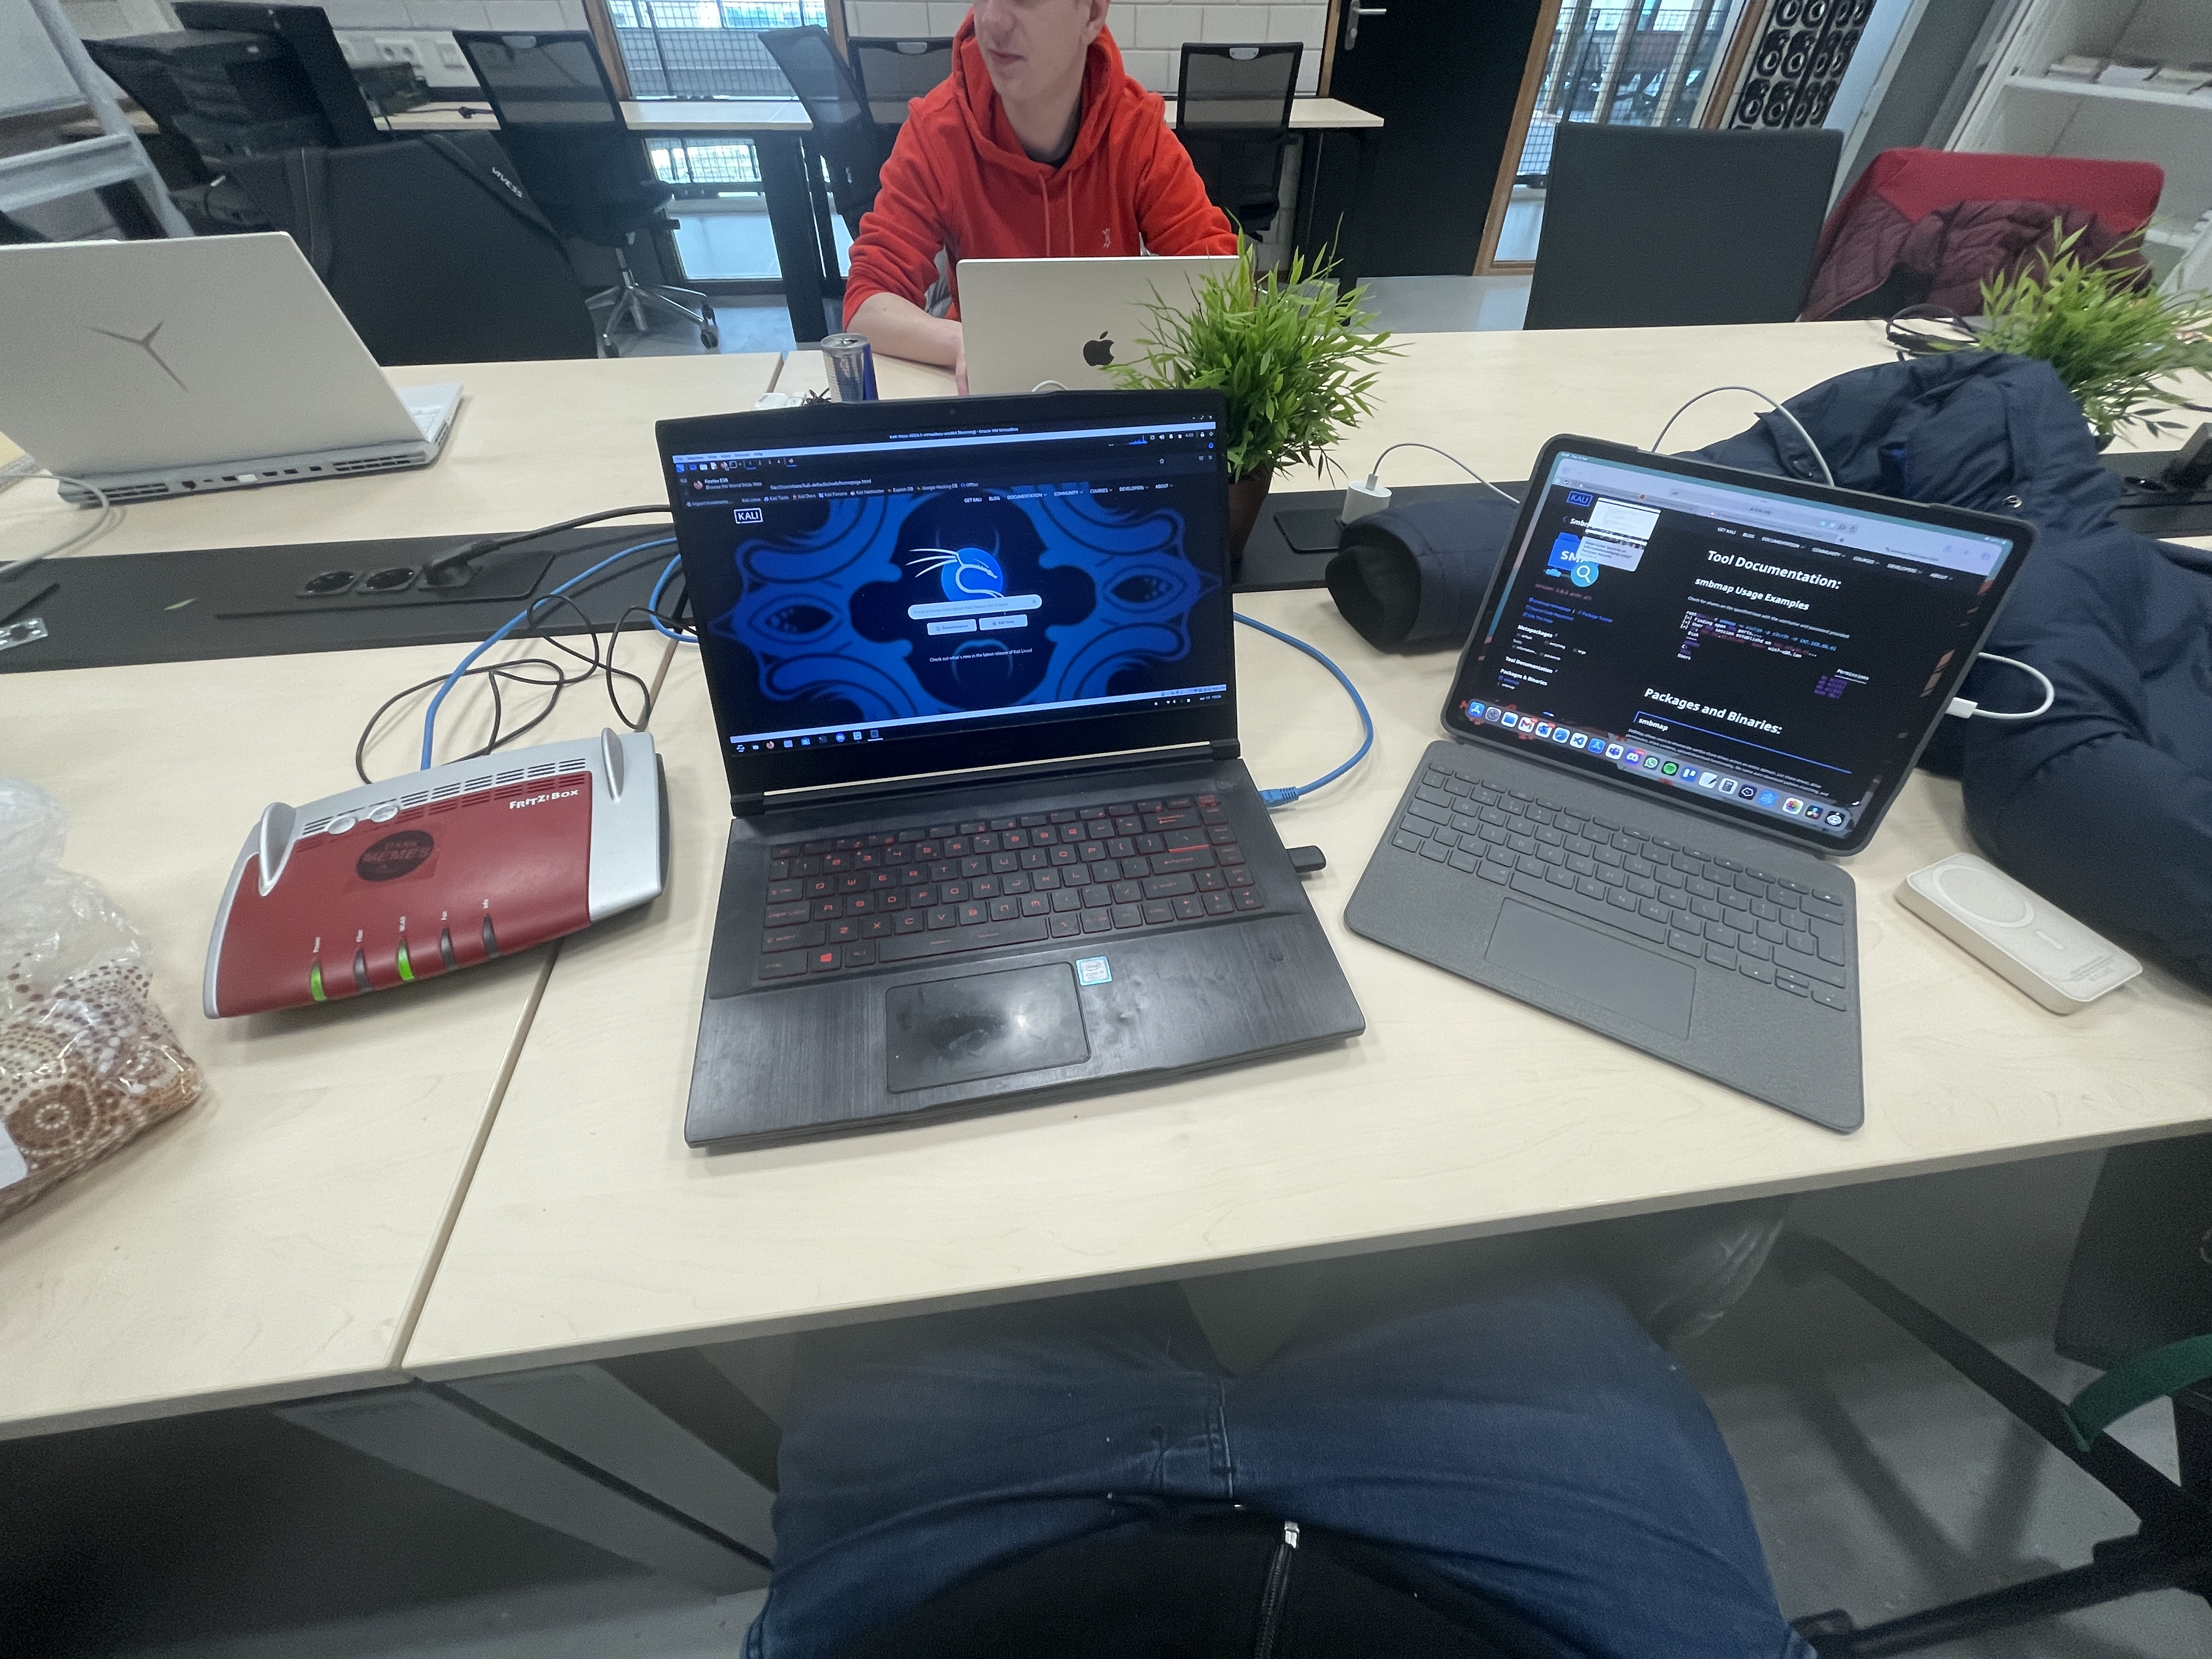
\includegraphics[width=0.8\textwidth]{fotos/PVI/Demo fail.jpeg}
\break
\emph{1 router 1 laptop with Virtualbox and 1 tablet for documentation}
\hfill\break
\hfill\break
For some reason, it would refuse to work without internet access or from a provider. so I had to test it in my own home where my router has been set up and it has SMB configured to be accessed to the web page. So after setting up my VM (Windows Vista Enterprise 32-bit)

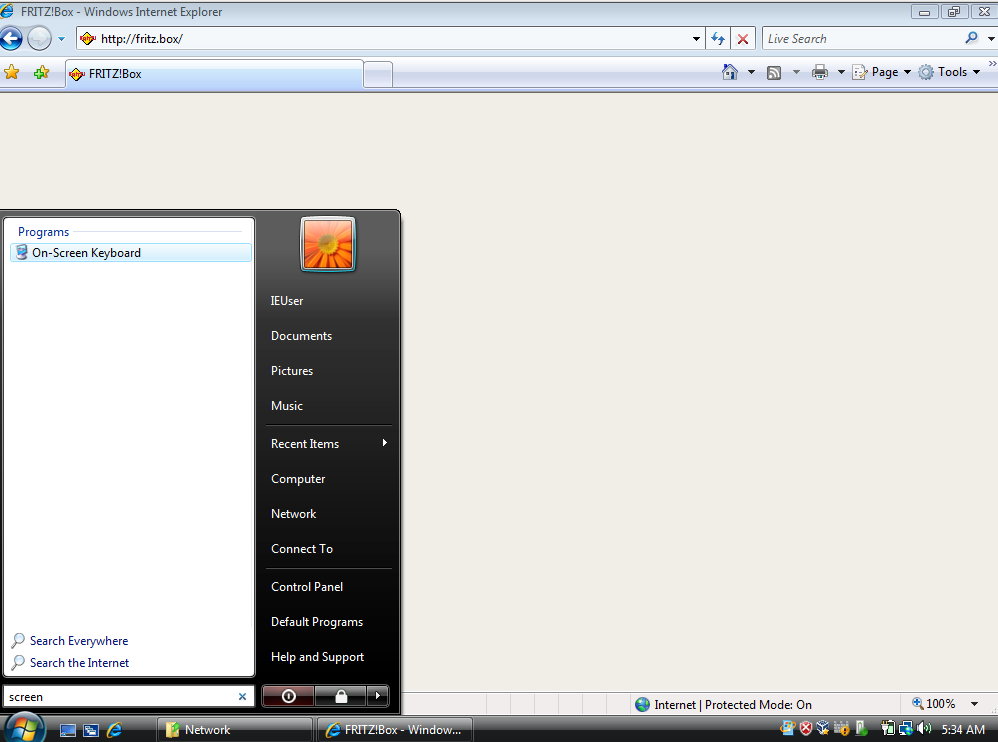
\includegraphics[width=0.8\textwidth]{fotos/PVI/Windows Vista/fritzbox was not loading vista.png}
\break
\emph{Trying to look if there was a connection to FRITZ using Internet Explorer 7}
\hfill\break
\hfill\break
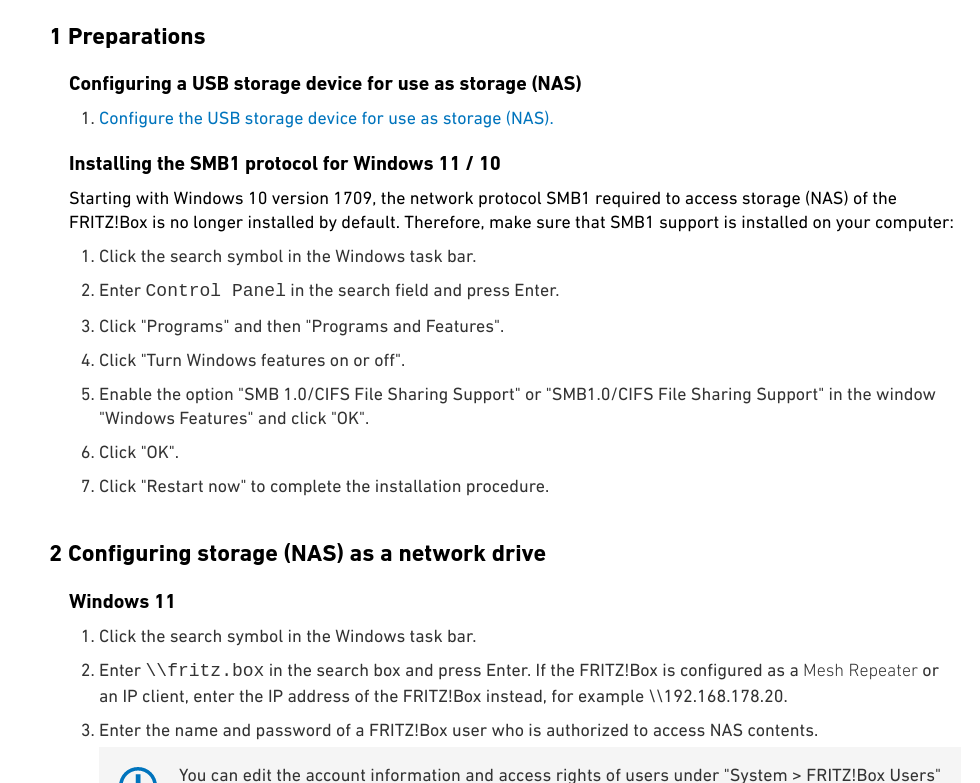
\includegraphics[width=0.8\textwidth]{fotos/PVI/Windows Vista/fritzbox setup.png}
\break
\emph{Looking up how to connect with Windows Vista to SMB. Since I don't need to enable SMB 1.0 I could skip to connecting to the NAS}
\hfill\break
\hfill\break
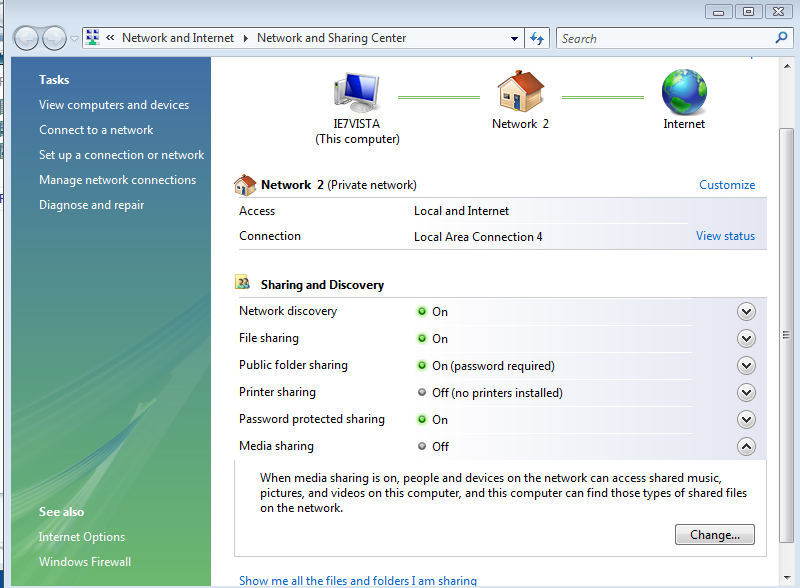
\includegraphics[width=0.8\textwidth]{fotos/PVI/Windows Vista/windos vista sharing center.png}
\break
\emph{We need to turn on our Network Discovery and sharing in Windows Vista}
\hfill\break
\hfill\break
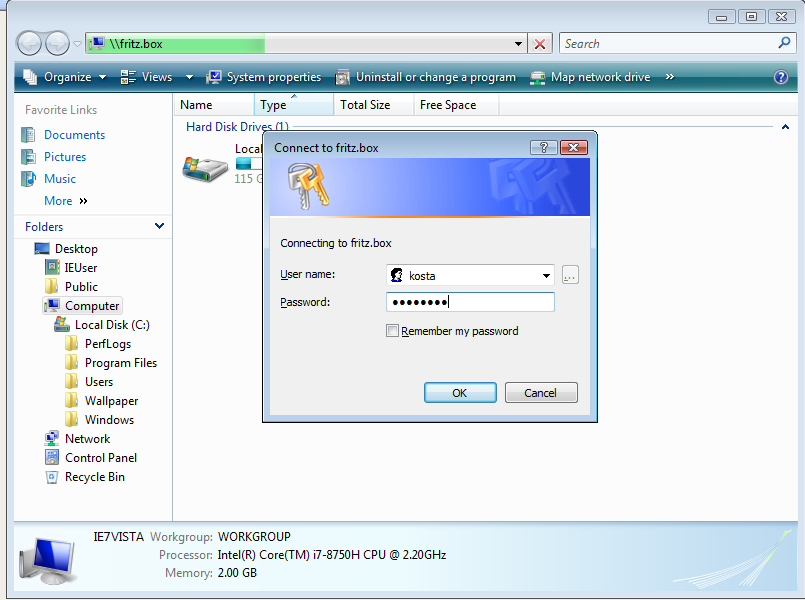
\includegraphics[width=0.8\textwidth]{fotos/PVI/Windows Vista/login smb fritz.png}
\break
\emph{Succes! It is trying to ask my fritznas password}
\hfill\break
\hfill\break
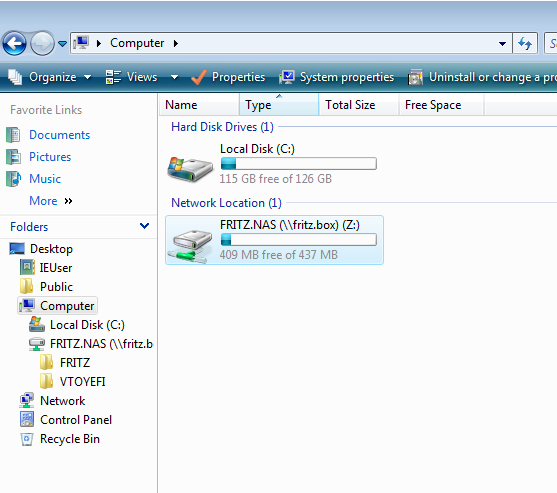
\includegraphics[width=0.8\textwidth]{fotos/PVI/Windows Vista/mapped fritznas.png}
\break
\emph{Adding my smb to a letter drive}
\hfill\break
\hfill\break
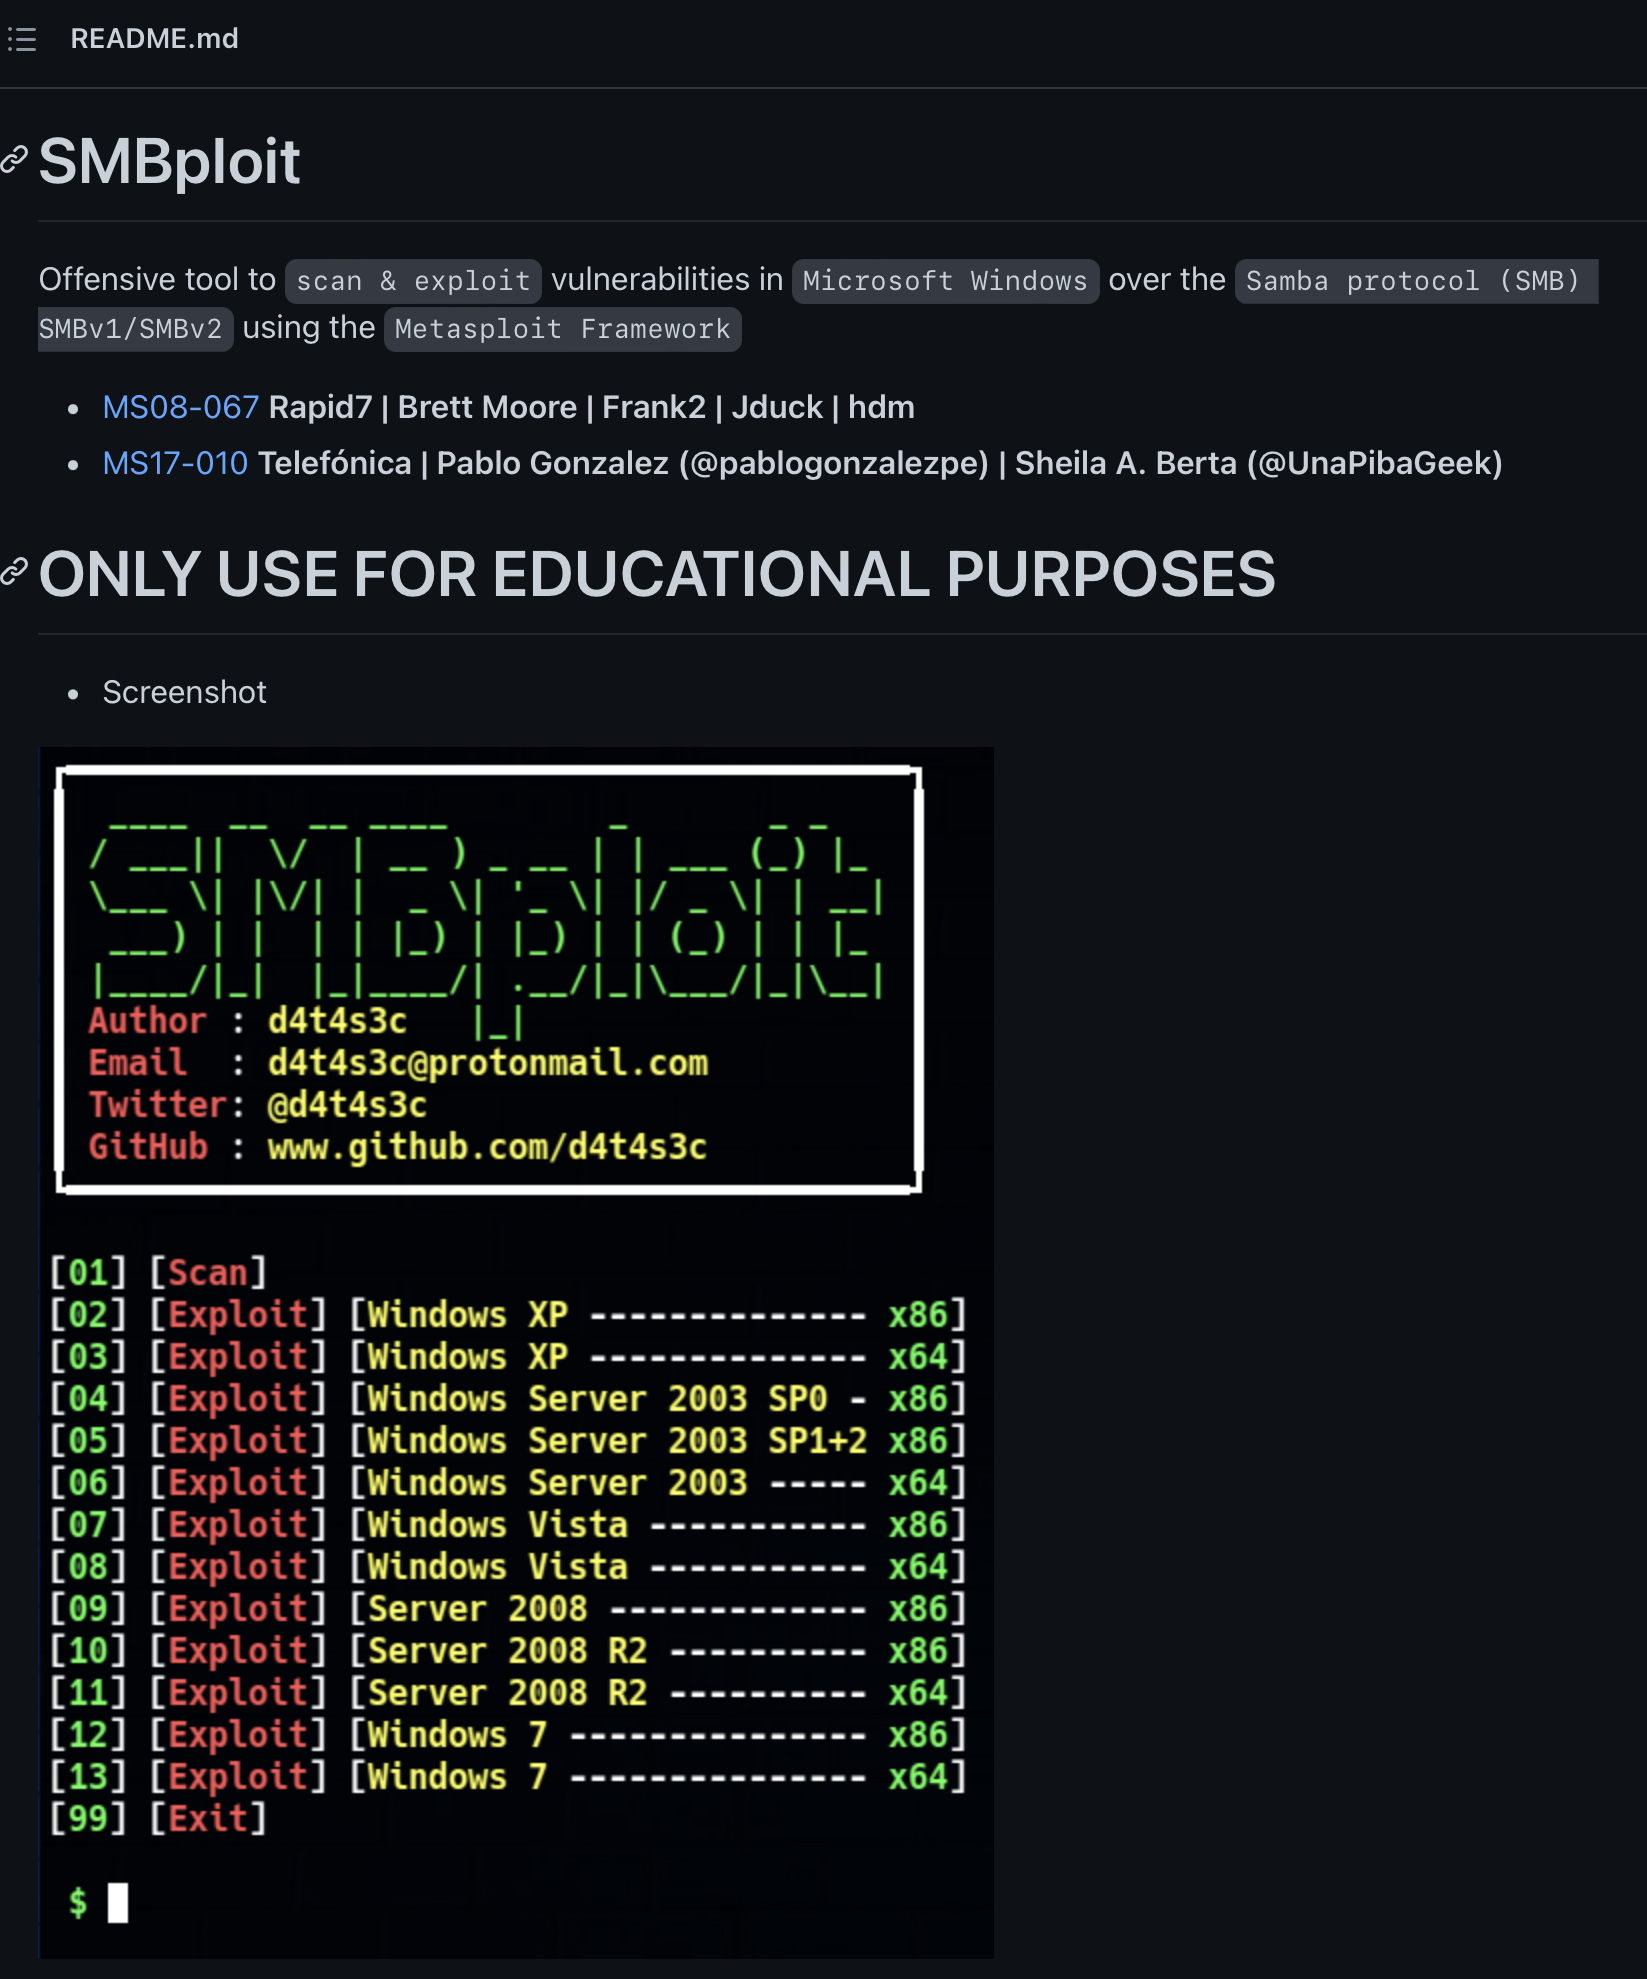
\includegraphics[width=0.8\textwidth]{fotos/PVI/Windows Vista/Github smbploit.jpeg}
\break
\emph{This is the tool I'm going to use since it uses EternalBlue}
\hfill\break
\hfill\break
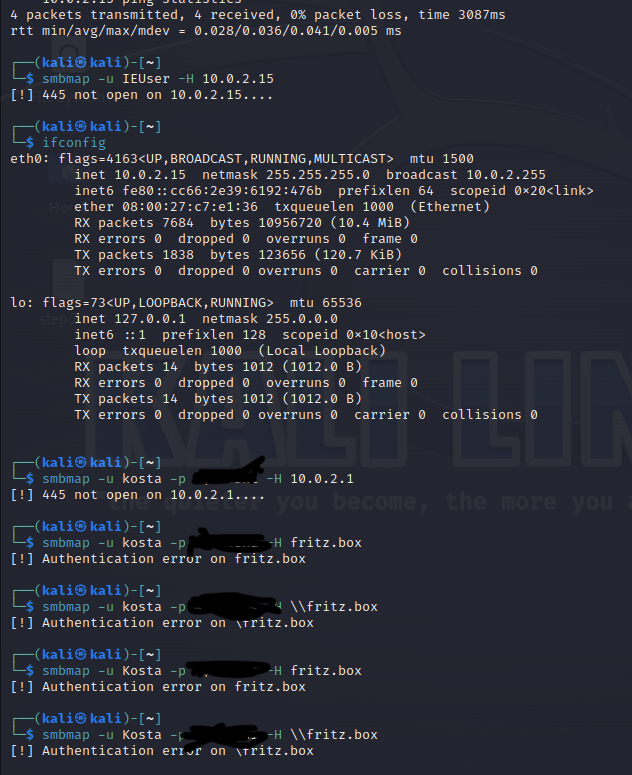
\includegraphics[width=0.8\textwidth]{fotos/PVI/Windows Vista/auth issue smbmap.png}
\break
\emph{Trying to map my main router NAS with my trusted credentials but it fails to connect}
\hfill\break
\hfill\break
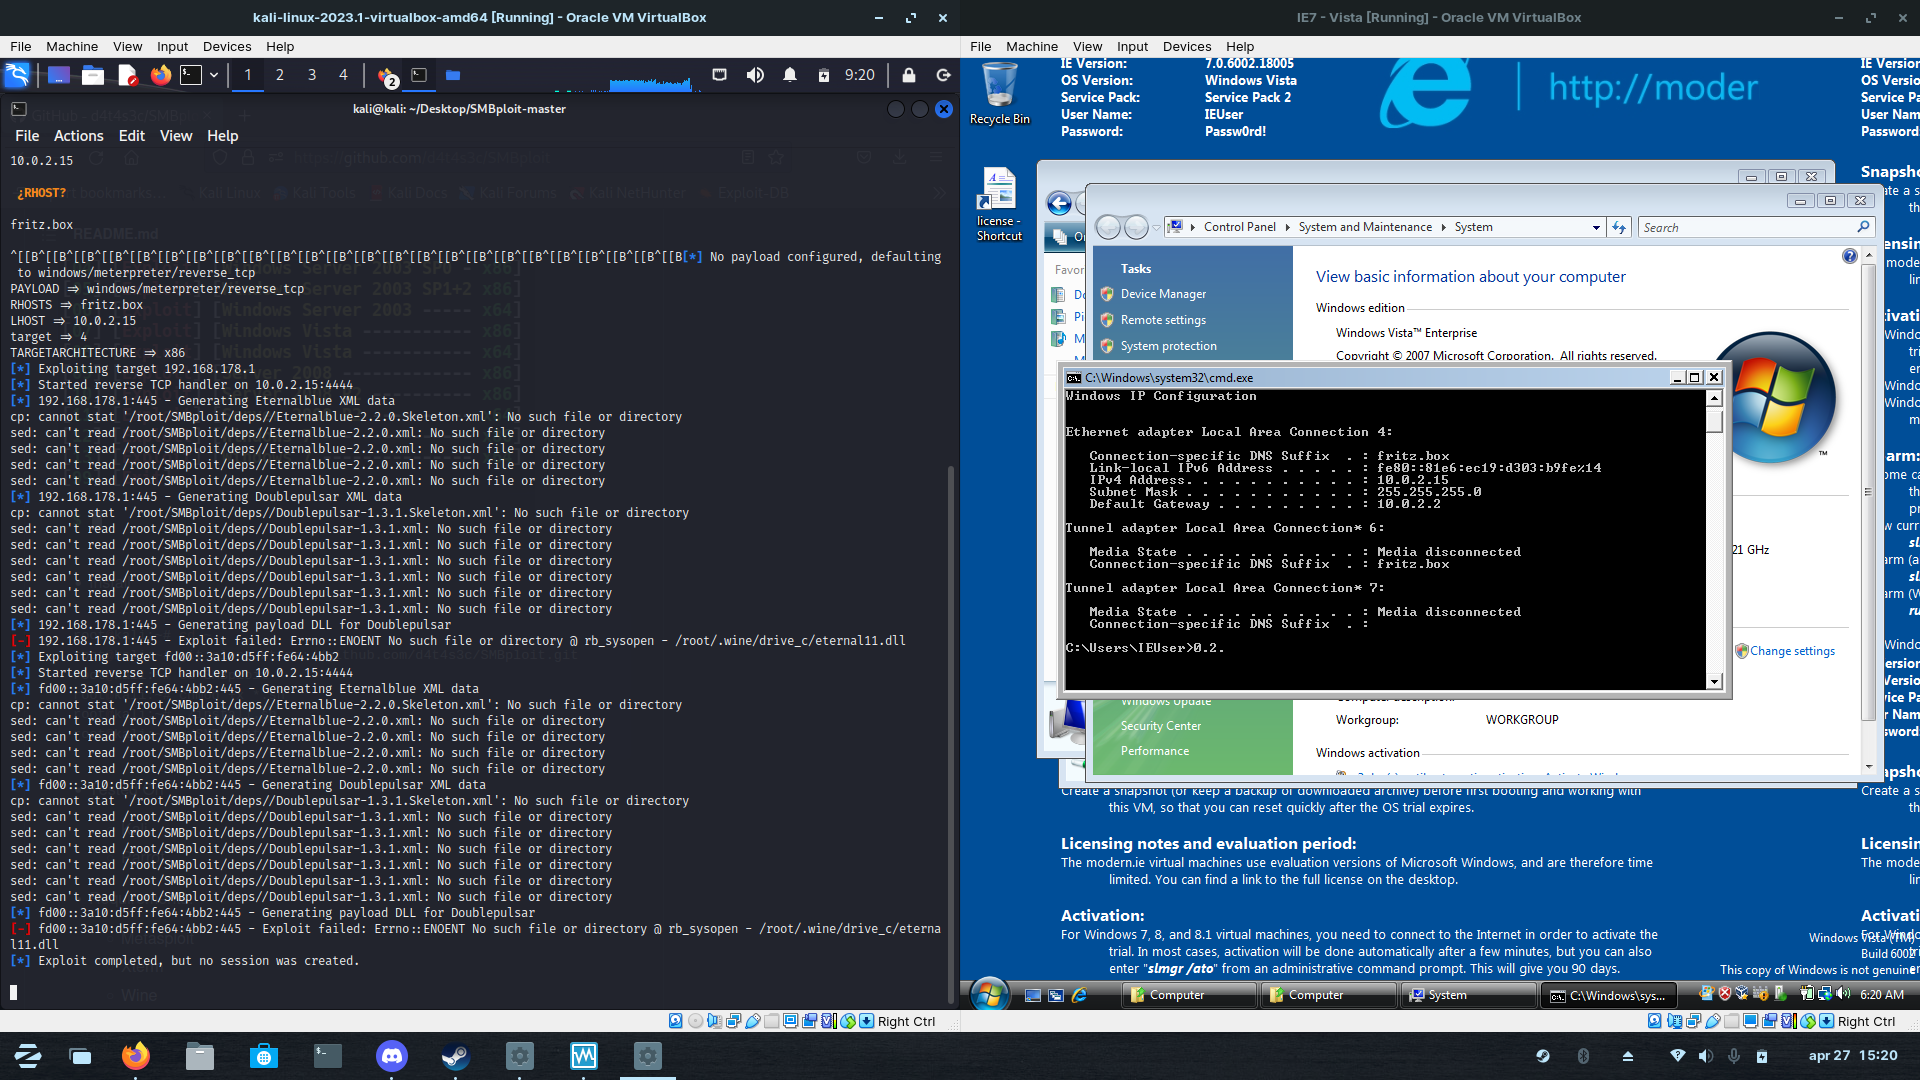
\includegraphics[width=0.9\textwidth]{fotos/PVI/Windows Vista/smbploit failed.png}
\break
\emph{Even with the right credentials it still fails}
\hfill\break
\hfill\break
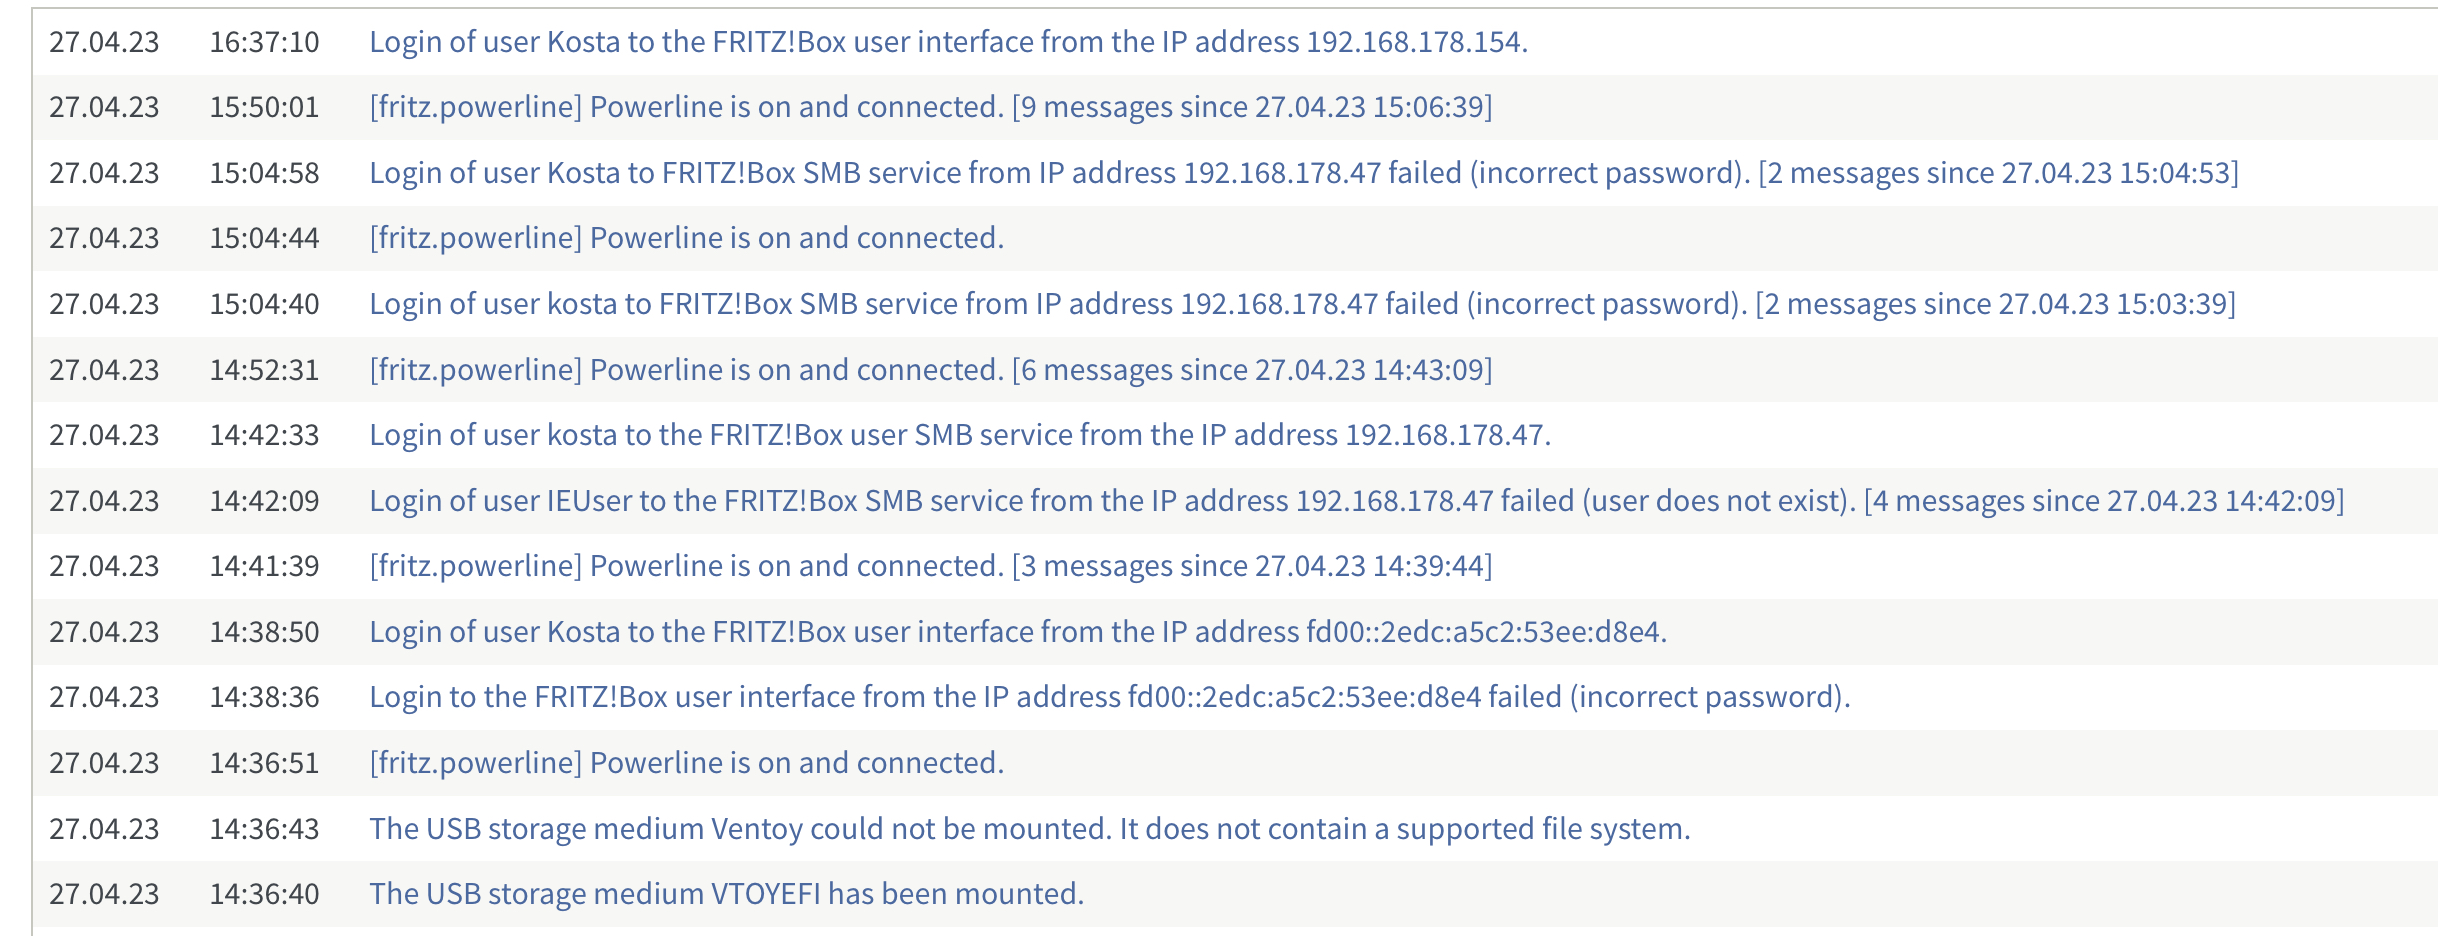
\includegraphics[width=1\textwidth]{fotos/PVI/Fritzbox/Logs.jpeg}
\break
\emph{My fritzbox did not like it at all but strange that it showed that it was the wrong password}

\newpage

\subsubsection{What have we found out}
For some reason, it keeps failing on me with errors that it cannot intercept even though the ping works correctly and they both can access to my NAS with Samba/SMB. Since my FRITZ!Box is running on the latest operating software which was updated last month. Yeah, old fritzboxes are still getting updates to this day. The logs aren't useful at all because it redirects me to AVM wiki explaining the basics. Even though I logged in to my NAS account multiple times in the same hour which would not be an issue. My test failed but your results may very. Maybe using an older router which is discontinued can yield more success. I've chosen Windows Vista just because it uses SMBv2 and SMBv1 as a backup. But my conclusion is that it does not pass my router securities to even send it to my Vista.
\newpage

\section{Outcomes}
Here I'll outline the outcomes of my investigation. What I'm hoping to achieve is to identify the exploit and suggest a solution to my classmates.

\subsection{Expected Outcomes}
My expectation will be set to low since SMB exploits are either patched or disabled by default in today's software.

But with older systems until Windows 7 - 8 it is possible just to crack and I think with the tool from Kali (submap) we can crack it in a few minutes and receive the files on NAS plus we can access the other host who are directly connected to the NAS

\subsection{Actual Outcomes}
I started to use my laptop and try my second FRITZ!Box (that I don't use) without access to the internet but my Kali refused to connect to my FRITZ!Box router is not even on the login screen of the device.
\hfill\break
\hfill\break
I tried it at home where my main router is located with everything working and my NAS ready to deploy. I've set everything online. And tried to use SMB map to scan 2 hosts connecting to each other with SMB e.g. Windows Vista and FRITZ!NAS through SMBv1. For some reason, it would not find anything. The second software that I used on my Kali was a Github script which is called SMBploit from d4t4s3c in GitHub. It came with its own issues but was managed to install it. After setting that this is Windows Vista running on 32-bit It was ready to run and still no success.
\newpage
\textbf{This was my setup for my testing}
\hfill\break
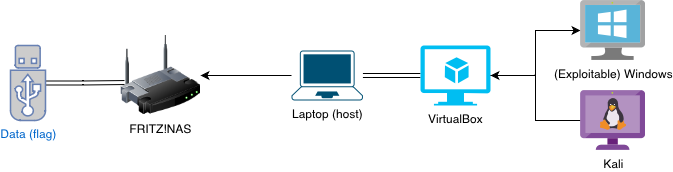
\includegraphics[width=1\textwidth]{fotos/PVI/PVI drawing.drawio.png}
\break
\emph{My drawing how I'm going to test my PVI}
\hfill\break
\hfill\break
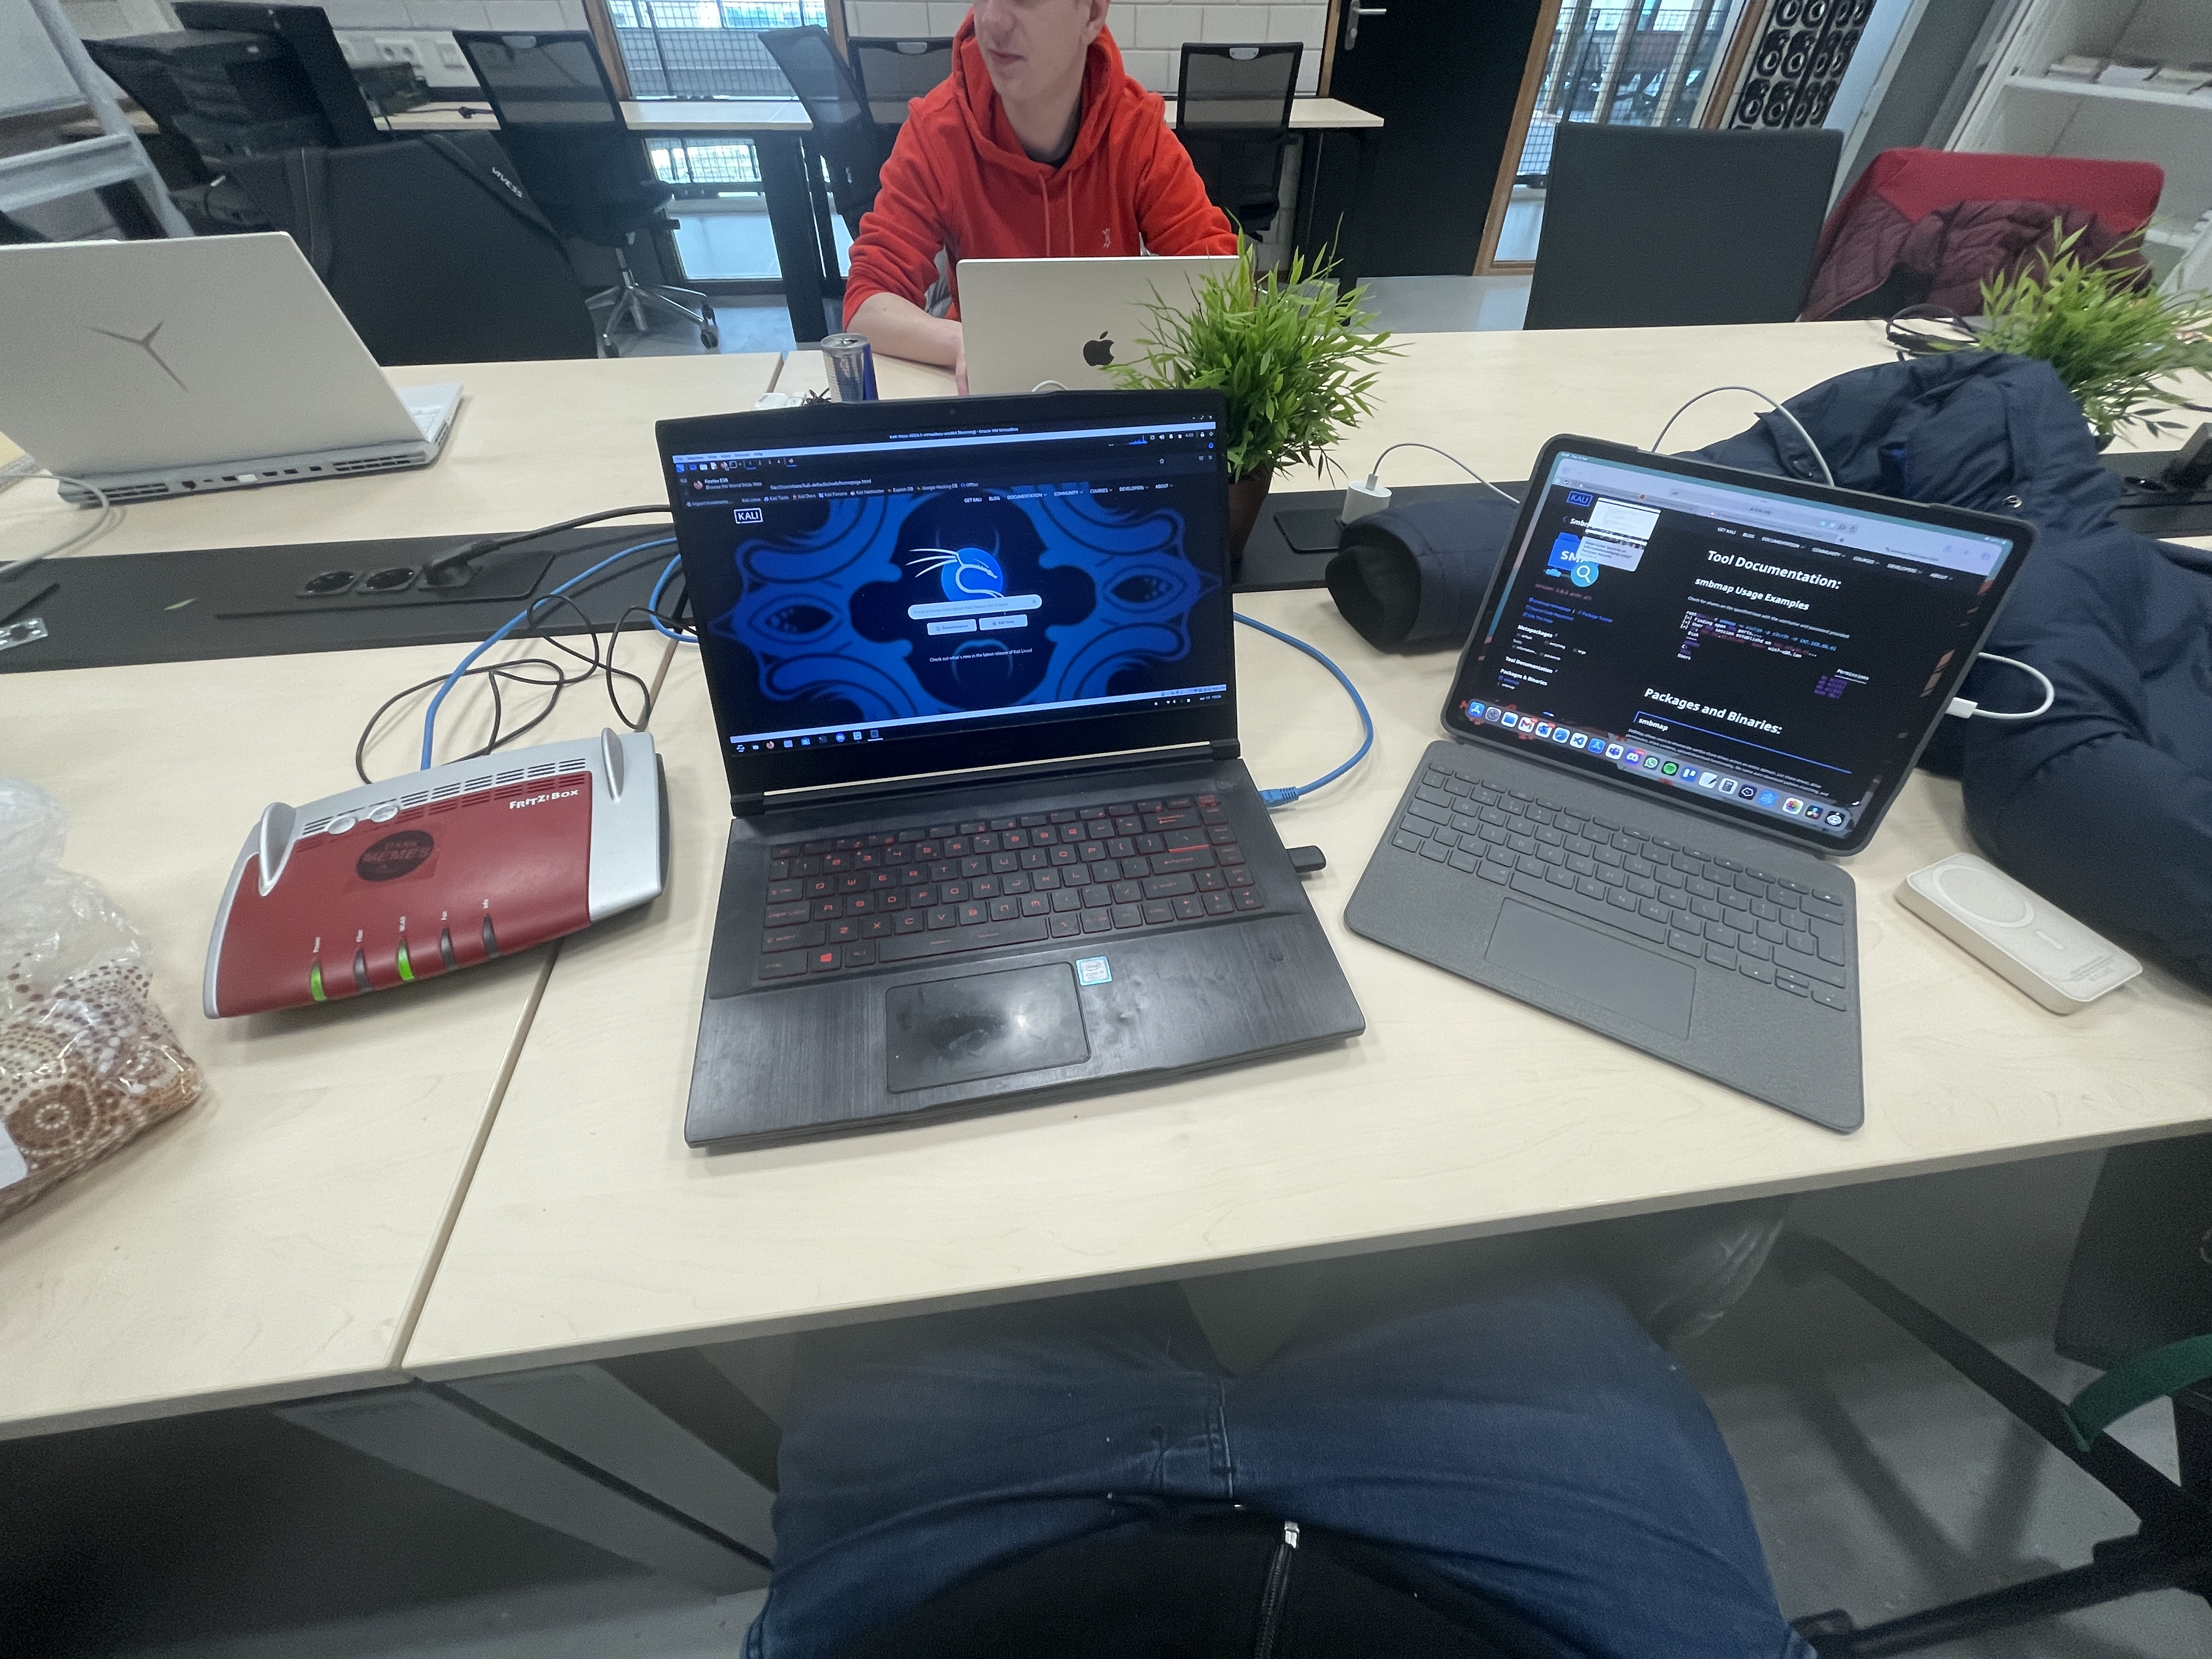
\includegraphics[width=0.8\textwidth]{fotos/PVI/Demo fail.jpeg}
\break
\emph{1 router 1 laptop with Virtualbox and 1 tablet for documentation}
\hfill\break
\hfill\break
I will ask if Dean can help me or if I can borrow his equipment.

\newpage
\section{Planning}
In this section I'm going to plan my estimated times:
\hfill\break
    \begin{table}[htbp]
        \begin{tabular}{|l|l|l|}
            \hline
            Estimate Hours & Activity    & Personnel    \tabularnewline \hline
            5 - 10 hours   & Researching about the subject & Kosta \tabularnewline \hline
            2 - 5 hours  & Document my investigation & Kosta \tabularnewline 
            \hline
            10 - 15 hours & Run it in my test environment & Kosta \tabularnewline \hline
            2 - 5 hours & Create Presentation & Kosta \tabularnewline \hline
        \end{tabular}
    \end{table}

\section{Conclusion}
Conclusion? Conclusion! The conclusion is that there are a lot of exploits but it is only focused on.

\hfill\break
Based on the research that I've conducted, it is clear that SMBv1 or SMB 1 poses significant security risks due to the numerous vulnerabilities that have been discovered over the years. Exploits and malware have shown how dangerous SMBv1 can be, as they can lead to the compromise of sensitive data, unauthorized access to systems, and the installation of additional malware. It is important to note that devices that use SMBv1, including older Windows machines

\hfill\break
Although FRITZ!Box and FRITZ!NAS devices are known to support SMBv1, there is a lack of documented CVEs that specifically focus on these devices. This suggests that any testing done to exploit SMBv1 on these devices has not been publicly disclosed. As a precautionary measure, it is recommended to disable SMBv1 and use more secure versions of the protocol to reduce the risk of exploitation. Overall, it is crucial to stay up to date with the latest security measures to ensure the confidentiality, integrity, and availability of sensitive data.

\newpage
\subsection{About the Research Questions}
Based on the limited information that I've found. It looks like AVM has mitigated most of the threats that exist in SMB exploits. We saw that there are 3 big exploits used on SMBv1 and they are EternalBlue, SambaCry and Badlock. The CVEs can be looked at in "Sub Research questions". This affects confidentiality and integrity the most the availability is also compromised but it is not the goal of these exploits. At least what it was initially built for, because the hacker has his own motives/intentions we would not understand what they going to do with these exploits. 

\hfill\break
Even if these exploits impose any thread most devices either do not support it anymore or are patched and it is hard to impossible for some devices since they are made in embedded Linux and are patched with SAMBA which means remote executions are not possible on the NAS itself. So I conclude that the Modern SMB/Samba/Netsmb are safe because we take into account that transfers mandate security like encryption, handshake and use of TCP.

\end{document}
